% =======================================================================================================
\section{Fundamentos da rede perceptron multicamadas}
\label{sec:mlp}

Esta seção constrói a MLP do zero. A ideia é que cada fórmula tenha uma interpretação e que o
leitor possa, ao final, implementar a rede em qualquer linguagem. A derivação completa da
retropropagação, com todas as passagens, está no Apêndice~\ref{ap:backprop}.

\subsection{Do neurônio artificial ao perceptron}

O modelo de McCulloch e Pitts \cite{mcculloch1943} descreve um neurônio como uma unidade que soma
entradas ponderadas e aplica um limiar. Em notação vetorial, com entradas
$\bx = (x_1,\dots,x_d)\T$, pesos $\bm{w} = (w_1,\dots,w_d)\T$ e viés $b$:

\begin{equation}
	z = \bm{w}\T \bx + b = \sum_{j=1}^{d} w_j x_j + b,
	\qquad
	a = f(z),
	\label{eq:neuronio}
\end{equation}

em que $f$ é a função de ativação. A \figura{fig:neuronio} representa essa unidade. O viés $b$
desempenha o papel de um peso associado a uma entrada constante igual a $1$; ele desloca a
fronteira de decisão e permite que ela não passe pela origem.

\begin{figure}[htbp]
	\centering
	\begin{tikzpicture}[>=Stealth,font=\small,node distance=8mm]
		\node (x1) at (0,1.9) {$x_1$};
		\node (x2) at (0,1.1) {$x_2$};
		\node (x3) at (0,0.3) {$\vdots$};
		\node (x4) at (0,-0.5) {$x_d$};
		\node[circle,draw,thick,minimum size=13mm,fill=blue!8] (soma) at (3.6,0.7) {$\Sigma$};
		\node[draw,thick,rounded corners=2pt,minimum width=13mm,minimum height=11mm,
		fill=orange!15] (ativ) at (5.6,0.7) {$f$};
		\node (saida) at (7.9,0.7) {$a = f(\bm{w}\T\bx+b)$};
		\node[circle,draw,minimum size=6mm,fill=gray!12] (bias) at (3.6,2.4) {$1$};
		\draw[->] (x1) -- node[above,font=\scriptsize,pos=0.45] {$w_1$} (soma);
		\draw[->] (x2) -- node[above,font=\scriptsize,pos=0.45] {$w_2$} (soma);
		\draw[->] (x3) -- node[above,font=\scriptsize,pos=0.5] {$\vdots$} (soma);
		\draw[->] (x4) -- node[below,font=\scriptsize,pos=0.45] {$w_d$} (soma);
		\draw[->] (bias) -- node[right,font=\scriptsize] {$b$} (soma);
		\draw[->,thick] (soma) -- node[above,font=\scriptsize] {$z$} (ativ);
		\draw[->,thick] (ativ) -- (saida);
		\node[font=\scriptsize,gray] at (0,-1.1) {entradas};
		\node[font=\scriptsize,gray] at (3.6,3.1) {viés};
	\end{tikzpicture}
	\caption{Unidade de um neurônio artificial: combinação linear das entradas seguida de uma
	ativação não linear. O viés $b$ é uma entrada constante que desloca o limiar de ativação.}
	\label{fig:neuronio}
\end{figure}

Um único neurônio com ativação degrau é o perceptron de Rosenblatt \cite{rosenblatt1958}. Sua
capacidade é limitada: ele só resolve problemas linearmente separáveis, e o contraexemplo clássico
é a função lógica XOR \cite{minsky1969}. A saída para essa limitação não é um neurônio mais
complexo, mas uma \emph{composição} de neurônios: a rede.

\subsection{Arquitetura e propagação direta}

Uma MLP organiza os neurônios em camadas. A camada $0$ é a entrada (os atributos), a camada $L$ é a
saída e as camadas $1,\dots,L-1$ são ocultas. Sejam $n_l$ o número de neurônios da camada $l$,
$\bW^{(l)} \in \R^{n_{l-1}\times n_l}$ a matriz de pesos que liga a camada $l-1$ à camada $l$ e
$\bb^{(l)} \in \R^{n_l}$ o vetor de vieses.

Com $m$ amostras organizadas em uma matriz $\bX \in \R^{m\times d}$ (uma amostra por linha), a
propagação direta é

\begin{align}
	\bA^{(0)} &= \bX, \label{eq:forward-a0}\\
	\bZ^{(l)} &= \bA^{(l-1)} \bW^{(l)} + \mathbf{1}_m \bb^{(l)\top},
	\qquad l = 1,\dots,L, \label{eq:forward-z}\\
	\bA^{(l)} &= f_l\!\left(\bZ^{(l)}\right),
	\qquad l = 1,\dots,L-1, \label{eq:forward-a}
\end{align}

em que $\mathbf{1}_m$ é o vetor de $m$ uns (o mesmo viés para todas as amostras) e $f_l$ é aplicada
elemento a elemento. Na saída, para classificação multiclasse, usa-se a função \emph{softmax}:

\begin{equation}
	p_{ik} = \frac{\exp\!\left(z_{ik}^{(L)}\right)}{\displaystyle\sum_{j=1}^{C}\exp\!\left(z_{ij}^{(L)}\right)},
	\qquad k = 1,\dots,C,
	\label{eq:softmax}
\end{equation}

com $C$ classes. A saída $\bp_i = (p_{i1},\dots,p_{iC})$ é uma distribuição de probabilidade sobre
as classes, e a previsão é $\hat{y}_i = \argmax_k p_{ik}$.

A \figura{fig:arquitetura} mostra a arquitetura usada como referência neste relatório, com quatro
entradas, duas camadas ocultas e três saídas. Cada ligação é um parâmetro a estimar.

\begin{figure}[htbp]
	\centering
	\begin{tikzpicture}[>=Stealth,font=\scriptsize,scale=0.95,transform shape]
		\def\dy{0.85}
		% entrada
		\foreach \i/\n in {1/x_1,2/x_2,3/x_3,4/x_4}{
			\node[circle,draw,thick,minimum size=0.62cm,fill=blue!10] (I\i) at (0,{(4.5-\i)*\dy}) {$\n$};
		}
		% oculta 1 (5 neurônios)
		\foreach \j in {1,...,5}{
			\node[circle,draw,thick,minimum size=0.62cm,fill=orange!15] (H1\j) at (2.9,{(5.5-\j)*\dy}) {};
		}
		% oculta 2 (4 neurônios)
		\foreach \k in {1,...,4}{
			\node[circle,draw,thick,minimum size=0.62cm,fill=orange!15] (H2\k) at (5.8,{(5-\k)*\dy}) {};
		}
		% saída
		\foreach \o/\n in {1/y_1,2/y_2,3/y_3}{
			\node[circle,draw,thick,minimum size=0.62cm,fill=green!12] (O\o) at (8.7,{(4-\o)*\dy}) {$\n$};
		}
		% vieses
		\node[circle,draw,minimum size=0.45cm,fill=gray!20] (B1) at (2.9,4.9) {$1$};
		\node[circle,draw,minimum size=0.45cm,fill=gray!20] (B2) at (5.8,4.4) {$1$};
		% conexões
		\foreach \i in {1,...,4} \foreach \j in {1,...,5} \draw[gray!55,line width=0.25pt] (I\i) -- (H1\j);
		\foreach \j in {1,...,5} \foreach \k in {1,...,4} \draw[gray!55,line width=0.25pt] (H1\j) -- (H2\k);
		\foreach \k in {1,...,4} \foreach \o in {1,...,3} \draw[gray!55,line width=0.25pt] (H2\k) -- (O\o);
		\foreach \j in {1,...,5} \draw[gray!80,dashed] (B1) -- (H1\j);
		\foreach \k in {1,...,4} \draw[gray!80,dashed] (B2) -- (H2\k);
		% rótulos
		\node[font=\scriptsize,above] at (0,3.1) {entrada};
		\node[font=\scriptsize,above] at (2.9,4.2) {oculta 1};
		\node[font=\scriptsize,above] at (5.8,3.65) {oculta 2};
		\node[font=\scriptsize,above] at (8.7,2.9) {saída};
		\node[font=\scriptsize,below] at (1.45,0.55) {$\bW^{(1)}$};
		\node[font=\scriptsize,below] at (4.35,0.55) {$\bW^{(2)}$};
		\node[font=\scriptsize,below] at (7.25,0.55) {$\bW^{(3)}$};
		\node[font=\scriptsize,above,gray] at (0,-0.55) {$d=4$};
		\node[font=\scriptsize,above,gray] at (2.9,-0.55) {$n_1=5$};
		\node[font=\scriptsize,above,gray] at (5.8,-0.9) {$n_2=4$};
		\node[font=\scriptsize,above,gray] at (8.7,-1.3) {$C=3$};
	\end{tikzpicture}
	\caption{Arquitetura de uma MLP com duas camadas ocultas. As linhas tracejadas representam os
	vieses, que funcionam como neurônios de entrada fixos em $1$.}
	\label{fig:arquitetura}
\end{figure}

\paragraph{Contagem de parâmetros.} Cada camada $l$ contribui com $n_{l-1}n_l$ pesos e $n_l$
vieses. Para a arquitetura $4$--$16$--$3$ adotada neste relatório:
\begin{equation}
	\underbrace{4 \times 16 + 16}_{\text{camada oculta}} \;+\;
	\underbrace{16 \times 3 + 3}_{\text{camada de saída}} = 64 + 16 + 48 + 3 = 131
	\label{eq:parametros}
\end{equation}
parâmetros, valor confirmado em execução (\parametrosMLP{}). A rede $4$--$5$--$4$--$3$ da
\figura{fig:arquitetura} teria $4\cdot5+5 + 5\cdot4+4 + 4\cdot3+3 = 20+5+20+4+12+3 = 64$
parâmetros. Comparar o número de parâmetros com o número de amostras é o primeiro teste de
viabilidade: com 150 amostras, uma rede com dezenas de milhares de parâmetros não tem como ser
estimada de forma confiável.

\subsection{Funções de ativação}

A não linearidade é o que distingue a MLP de uma regressão logística. Sem ela, a composição de
camadas colapsa em uma única transformação afim: $\bW^{(2)}f(\bW^{(1)}\bx) = \bW'\bx$ se $f$ é
linear. As funções mais usadas estão na \tabela{tab:ativacoes-math} e na
\figura{fig:ativacoes-curvas}.

\begin{table}[htbp]
	\centering
	\caption{Funções de ativação usuais, derivadas e faixa de saída.}
	\label{tab:ativacoes-math}
	\small
	\begin{tabular}{L{2.6cm} L{4.2cm} L{4.3cm} L{2.4cm}}
		\toprule
		\textbf{Nome} & \textbf{Função $f(z)$} & \textbf{Derivada $f'(z)$} & \textbf{Faixa} \\
		\midrule
		Identidade & $z$ & $1$ & $(-\infty,\infty)$ \\
		Logística (sigmoide) & $\dfrac{1}{1+e^{-z}}$ & $f(z)\left(1-f(z)\right)$ & $(0,1)$ \\
		Tangente hiperbólica & $\tanh(z) = \dfrac{e^{z}-e^{-z}}{e^{z}+e^{-z}}$ & $1-\tanh^2(z)$ & $(-1,1)$ \\
		ReLU & $\max(0,z)$ & $\indic[z>0]$ & $[0,\infty)$ \\
		Leaky ReLU & $\max(\alpha z, z)$ & $1$ se $z>0$; $\alpha$ caso contrário & $(-\infty,\infty)$ \\
		Softmax (saída) & $\dfrac{e^{z_k}}{\sum_j e^{z_j}}$ & ver \equacao{eq:softmax-jacobiano} & $(0,1)$ \\
		\bottomrule
	\end{tabular}
\end{table}

\begin{figure}[htbp]
	\centering
	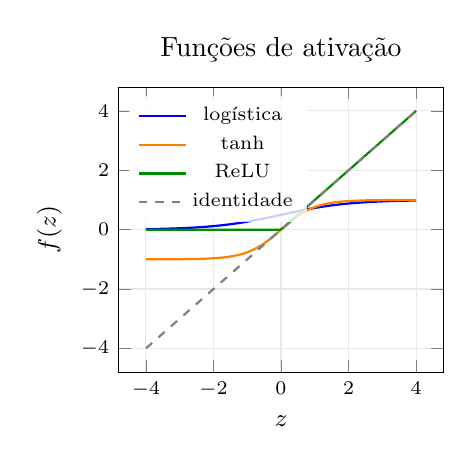
\begin{tikzpicture}
		\begin{axis}[
			width=0.47\textwidth, height=5.2cm,
			xlabel={$z$}, ylabel={$f(z)$},
			domain=-4:4, samples=120, grid=both, grid style={gray!18},
			legend pos=north west, legend style={font=\scriptsize,draw=none,fill=white,fill opacity=0.8,text opacity=1},
			tick label style={font=\scriptsize}, label style={font=\small},
			title={Funções de ativação},
		]
			\addplot[blue,thick] {1/(1+exp(-x))}; \addlegendentry{logística}
			\addplot[orange,thick] {tanh(x)}; \addlegendentry{tanh}
			\addplot[green!55!black,thick] {max(0,x)}; \addlegendentry{ReLU}
			\addplot[gray,dashed,thick] {x}; \addlegendentry{identidade}
		\end{axis}
	\end{tikzpicture}\hfill
	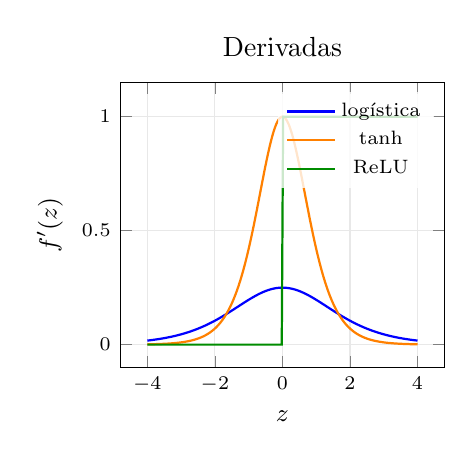
\begin{tikzpicture}
		\begin{axis}[
			width=0.47\textwidth, height=5.2cm,
			xlabel={$z$}, ylabel={$f'(z)$},
			domain=-4:4, samples=200, grid=both, grid style={gray!18},
			legend pos=north east, legend style={font=\scriptsize,draw=none,fill=white,fill opacity=0.8,text opacity=1},
			tick label style={font=\scriptsize}, label style={font=\small},
			title={Derivadas},
			ymin=-0.1, ymax=1.15,
		]
			\addplot[blue,thick] {exp(-x)/(1+exp(-x))^2}; \addlegendentry{logística}
			\addplot[orange,thick] {1-tanh(x)^2}; \addlegendentry{tanh}
			\addplot[green!55!black,thick] {x>0 ? 1 : 0}; \addlegendentry{ReLU}
		\end{axis}
	\end{tikzpicture}
	\caption{Funções de ativação e suas derivadas. A derivada da logística e a da tangente
	hiperbólica se aproximam de zero nas caudas --- a origem do problema de gradiente que
	desaparece. A ReLU tem derivada constante igual a $1$ para $z>0$, o que preserva o sinal do
	gradiente em redes profundas.}
	\label{fig:ativacoes-curvas}
\end{figure}

\paragraph{Escolha da ativação.} A ReLU é o padrão em redes profundas por ser barata e por não
saturar no lado positivo \cite{he2015}. A \emph{tanh} é simétrica em relação à origem e costuma
convergir bem em redes pequenas com dados padronizados --- é a escolha do modelo deste relatório.
A logística é historicamente importante, mas satura nos dois lados e, por isso, treina mais
devagar. A identidade não é uma não linearidade: usá-la na camada oculta equivale a um modelo
linear, o que, no Iris, é quase tão bom quanto a rede (ver \secao{sec:resultados}).

\paragraph{Por que não usar degrau.} A função degrau tem derivada nula em quase toda parte e
indefinida em zero. Sem gradiente, não há retropropagação. Foi exatamente essa dificuldade que
manteve as redes neurais adormecidas entre as décadas de 1970 e 1980.

\subsection{Camada de saída e função de custo}
\label{sec:custo}

Para classificação multiclasse, a saída natural é a softmax \equacao{eq:softmax} combinada com a
entropia cruzada categórica. Com os rótulos codificados em \emph{one-hot}
$\by_i \in \{0,1\}^{C}$ ($y_{ik}=1$ se a amostra $i$ pertence à classe $k$), a perda média é

\begin{equation}
	\Loss(\bW,\bb) = -\frac{1}{m}\sum_{i=1}^{m}\sum_{k=1}^{C} y_{ik}\,\log p_{ik}
	\;+\; \frac{\lambda}{2}\sum_{l=1}^{L}\left\|\bW^{(l)}\right\|_F^2,
	\label{eq:cross-entropy}
\end{equation}

em que $\|\cdot\|_F$ é a norma de Frobenius e $\lambda \ge 0$ controla a regularização $L_2$.
No scikit-learn, o hiperparâmetro \texttt{alpha} corresponde a $\lambda$ (a penalidade é somada
como $\alpha\|\bW\|^2/2$). O primeiro termo é a entropia cruzada: ele é mínimo quando a
probabilidade atribuída à classe correta é $1$, e cresce sem limite quando ela se aproxima de $0$.

\paragraph{A derivada que faz tudo funcionar.} A combinação softmax com entropia cruzada tem uma
propriedade notável. Para uma amostra isolada,

\begin{equation}
	\frac{\partial \Loss}{\partial z_k^{(L)}} = p_k - y_k, \qquad k = 1,\dots,C.
	\label{eq:softmax-grad}
\end{equation}

Ou seja: o gradiente em relação aos \emph{scores} de saída é simplesmente o erro de probabilidade.
A demonstração está no Apêndice~\ref{ap:backprop}, mas a intuição é direta. A softmax tem
jacobiano
\begin{equation}
	\frac{\partial p_k}{\partial z_j} = p_k\left(\delta_{kj} - p_j\right),
	\label{eq:softmax-jacobiano}
\end{equation}
e a regra da cadeia aplicada a $-\sum_k y_k \log p_k$ produz vários termos que se cancelam, porque
$\sum_k y_k = 1$ e $\sum_k p_k = 1$. O resultado \equacao{eq:softmax-grad} é a razão pela qual
essa combinação é onipresente.

\paragraph{Por que não erro quadrático.} Poderia parecer natural minimizar
$\frac{1}{2}\sum_k (p_k-y_k)^2$. Com a softmax, o gradiente resultante seria proporcional a
$p_k(1-p_k)$ e, quando a rede erra com confiança ($p_k \approx 0$ para a classe correta), esse fator
leva o gradiente a zero: o modelo erra muito e aprende pouco. Com a entropia cruzada, o gradiente
$p_k - y_k$ é máximo justamente quando o erro é maior. Além disso, a entropia cruzada é convexa
em relação aos \emph{scores} de saída (embora não em relação aos pesos da rede).

\paragraph{Regularização $L_2$.} O termo $\frac{\lambda}{2}\|\bW\|_F^2$ pune pesos grandes,
suavizando a função aprendida. Sua contribuição ao gradiente é $\lambda\bW$, o que dá origem ao
nome \emph{weight decay}: a cada passo, os pesos são encolhidos na direção da origem antes de
receberem o empurrão do erro. No scikit-learn, \texttt{alpha} é o $\lambda$ dessa formulação.

\subsection{Retropropagação}
\label{sec:backprop}

O objetivo do treinamento é encontrar $\bW,\bb$ que minimizem \equacao{eq:cross-entropy}. Como a
perda depende dos pesos de forma composicional, o gradiente é obtido pela regra da cadeia,
aplicada da saída para a entrada --- daí o nome \emph{retropropagação}
\cite{rumelhart1986}.

Defina o \emph{erro} da camada $l$ como a derivada da perda em relação à pré-ativação:
\begin{equation}
	\bm{\Delta}^{(l)} = \frac{\partial \Loss}{\partial \bZ^{(l)}} \in \R^{m\times n_l}.
	\label{eq:delta}
\end{equation}
Na saída, por \equacao{eq:softmax-grad},
\begin{equation}
	\bm{\Delta}^{(L)} = \frac{1}{m}\left(\bP - \bY\right).
	\label{eq:delta-L}
\end{equation}
Para as camadas ocultas, aplica-se a regra da cadeia duas vezes (uma para atravessar a ativação,
outra para atravessar a matriz de pesos):
\begin{equation}
	\bm{\Delta}^{(l)} = \left(\bm{\Delta}^{(l+1)}\bW^{(l+1)\top}\right) \odot f_l'\!\left(\bZ^{(l)}\right),
	\qquad l = L-1,\dots,1,
	\label{eq:delta-rec}
\end{equation}
em que $\odot$ é o produto de Hadamard (elemento a elemento). Com os erros de cada camada, os
gradientes dos parâmetros são

\begin{align}
	\frac{\partial \Loss}{\partial \bW^{(l)}} &= \bA^{(l-1)\top}\bm{\Delta}^{(l)} + \lambda\bW^{(l)},
	\label{eq:grad-W}\\
	\frac{\partial \Loss}{\partial \bb^{(l)}} &= \sum_{i=1}^{m}\bm{\Delta}^{(l)}_{i,:}
	= \mathbf{1}_m^{\top} \bm{\Delta}^{(l)}.
	\label{eq:grad-b}
\end{align}

A \figura{fig:fluxo-gradiente} resume o ciclo: a informação sobe pela rede (propagação direta), a
perda é calculada, e o erro desce pela rede (retropropagação) carregando, em cada camada, a
informação de quanto cada peso contribuiu para o erro final.

\begin{figure}[htbp]
	\centering
	\begin{tikzpicture}[>=Stealth,font=\small,node distance=10mm,
		caixa/.style={draw,thick,rounded corners=3pt,minimum height=9mm,align=center,fill=blue!6},
		seta/.style={->,thick}]
		\node[caixa] (x) {entrada\\$\bX$};
		\node[caixa,right=of x] (f) {propagação\\direta};
		\node[caixa,right=of f] (l) {perda\\$\Loss$};
		\node[caixa,below=of l] (g) {gradiente\\$\partial\Loss/\partial\bm{\theta}$};
		\node[caixa,left=of g] (b) {retro-\\propagação};
		\node[caixa,left=of b] (u) {atualização\\$\bm{\theta}\leftarrow\bm{\theta}-\eta\,\bm{g}$};
		\draw[seta] (x) -- (f);
		\draw[seta] (f) -- (l);
		\draw[seta] (l) -- (g);
		\draw[seta] (g) -- (b);
		\draw[seta] (b) -- (u);
		\draw[seta] (u) |- (f);
		\node[font=\scriptsize,gray,above] at (2.35,0.55) {pesos $\bm{\theta}$};
	\end{tikzpicture}
	\caption{Ciclo de treinamento. A propagação direta e a retropropagação têm o mesmo custo
	assintótico: $O\!\left(m\sum_l n_{l-1}n_l\right)$, isto é, proporcional ao número de
	parâmetros.}
	\label{fig:fluxo-gradiente}
\end{figure}

\paragraph{Custo computacional.} Uma passagem direta custa $O(m\sum_l n_{l-1}n_l)$ operações. A
retropropagação custa o mesmo, com uma constante pequena. Isso é decisivo: calcular o gradiente
por diferenças finitas custaria $O(P)$ passagens diretas, com $P$ o número de parâmetros, o que
seria inviável para redes reais. A retropropagação é o que torna o treinamento possível.

\paragraph{Verificação numérica.} Como a retropropagação é fácil de implementar errado, todo
código sério é validado por diferenças centrais:
\begin{equation}
	\frac{\partial \Loss}{\partial \theta_i} \approx
	\frac{\Loss(\theta_i+\varepsilon) - \Loss(\theta_i-\varepsilon)}{2\varepsilon},
	\qquad \varepsilon \approx 10^{-6},
	\label{eq:gradcheck}
\end{equation}
e compara-se com o gradiente analítico pelo erro relativo
$\left|g_{\text{ana}} - g_{\text{num}}\right| / \left(\left|g_{\text{ana}}\right| + \left|g_{\text{num}}\right|\right)$.
Valores abaixo de $10^{-4}$ indicam implementação correta. A
\figura{fig:gradiente} mostra o resultado obtido: erro máximo de \erroGrad{}, o que confirma a
derivação e o código.

\subsection{Otimização}
\label{sec:otimizacao}

Com o gradiente em mãos, o treinamento é um problema de otimização iterativa. A atualização mais
simples é o gradiente descendente:
\begin{equation}
	\bm{\theta}_{t+1} = \bm{\theta}_t - \eta\,\nabla_{\bm{\theta}}\Loss(\bm{\theta}_t),
	\label{eq:gd}
\end{equation}
com taxa de aprendizado $\eta > 0$. Calcular o gradiente com todas as $m$ amostras a cada passo é
caro e redundante; o \emph{gradiente descendente estocástico} (SGD) usa uma amostra ou um
\emph{minilote} $\mathcal{B}$ de tamanho $B$:
\begin{equation}
	\bm{\theta}_{t+1} = \bm{\theta}_t - \eta\,\widehat{\nabla}\Loss(\bm{\theta}_t),
	\qquad
	\widehat{\nabla}\Loss = \frac{1}{B}\sum_{i\in\mathcal{B}}\nabla \ell_i.
	\label{eq:sgd}
\end{equation}
O estimador é não viesado, mas ruidoso. Esse ruído, que à primeira vista parece um defeito, ajuda
a escapar de pontos de sela e de mínimos ruins.

\paragraph{Momento.} Para suavizar a trajetória, acumula-se uma velocidade:
\begin{align}
	\bm{v}_{t} &= \mu\,\bm{v}_{t-1} - \eta\,\bm{g}_t, \label{eq:momentum}\\
	\bm{\theta}_{t} &= \bm{\theta}_{t-1} + \bm{v}_{t}, \label{eq:momentum-upd}
\end{align}
com $\mu \in [0,1)$ (tipicamente $0{,}9$). A variante de Nesterov avalia o gradiente na posição
``adiantada'' $\bm{\theta} + \mu\bm{v}$, o que antecipa a correção.

\paragraph{Adam.} O otimizador Adam \cite{kingma2015} mantém médias móveis do gradiente e do
gradiente ao quadrado, com correção de viés:
\begin{align}
	\bm{m}_t &= \beta_1\bm{m}_{t-1} + (1-\beta_1)\bm{g}_t, \label{eq:adam-m}\\
	\bm{v}_t &= \beta_2\bm{v}_{t-1} + (1-\beta_2)\bm{g}_t^{\,2}, \label{eq:adam-v}\\
	\widehat{\bm{m}}_t &= \frac{\bm{m}_t}{1-\beta_1^{t}}, \qquad
	\widehat{\bm{v}}_t = \frac{\bm{v}_t}{1-\beta_2^{t}}, \label{eq:adam-bias}\\
	\bm{\theta}_t &= \bm{\theta}_{t-1} - \eta\,
	\frac{\widehat{\bm{m}}_t}{\sqrt{\widehat{\bm{v}}_t}+\epsilon},
	\label{eq:adam-upd}
\end{align}
com $\beta_1 = 0{,}9$, $\beta_2 = 0{,}999$ e $\epsilon = 10^{-8}$ como padrões. A divisão por
$\sqrt{\widehat{\bm{v}}}$ normaliza o passo por parâmetro: coordenadas com gradiente
sistematicamente grande recebem passos menores. É por isso que o Adam é bastante insensível à
escala dos atributos --- propriedade explorada no \secao{sec:resultados}.

\paragraph{Taxa de aprendizado.} É o hiperparâmetro mais importante. Taxa pequena faz o
treinamento lento e pode parar em região ruim; taxa grande faz a perda oscilar ou divergir. No
scikit-learn, o padrão de \texttt{MLPClassifier} é $\eta = 10^{-3}$ com Adam, e a taxa é reduzida
por $\eta_t = \eta_0 / t^{\,p}$ quando \texttt{learning\_rate='invscaling'}.

\subsection{Regularização e controle de capacidade}
\label{sec:regularizacao}

Um modelo com parâmetros demais ajusta o ruído do treino e generaliza mal. As técnicas de
regularização limitam essa capacidade de formas complementares.

\begin{itemize}
	\item \textbf{$L_2$ (weight decay)}: penaliza a norma dos pesos
	      \equacao{eq:cross-entropy}, mantendo-os pequenos e a função mais suave;
	\item \textbf{parada antecipada} (\emph{early stopping}): acompanha a perda em um conjunto de
	      validação e interrompe o treino quando ela para de melhorar, devolvendo os melhores pesos
	      \cite{prechelt1998}. No scikit-learn, isso é controlado por \texttt{early\_stopping},
	      \texttt{validation\_fraction} e \texttt{n\_iter\_no\_change};
	\item \textbf{\emph{dropout}}: durante o treino, desliga neurônios ao acaso com probabilidade
	      $q$, forçando representações redundantes \cite{srivastava2014}. Não é usado aqui, porque
	      com 150 amostras o efeito é mais ruído do que regularização;
	\item \textbf{aumento de dados}: não se aplica diretamente a medidas de flores, mas é a
	      regularização mais eficaz em imagens e áudio;
	\item \textbf{redução da arquitetura}: menos neurônios, menos parâmetros, menos variância.
\end{itemize}

\subsection{Inicialização}

Se todos os pesos começam iguais, todos os neurônios de uma camada recebem o mesmo gradiente e
permanecem idênticos --- a chamada quebra de simetria nunca ocorre. Por isso a inicialização é
aleatória, mas com variância calibrada para preservar a escala dos sinais entre camadas.

A inicialização de Xavier/Glorot \cite{glorot2010} escolhe
\begin{equation}
	\Var\!\left(W_{ij}^{(l)}\right) = \frac{2}{n_{l-1}+n_l},
	\label{eq:xavier}
\end{equation}
adequada para ativações simétricas como a \emph{tanh}. Para a ReLU, a inicialização de He
\cite{he2015} usa
\begin{equation}
	\Var\!\left(W_{ij}^{(l)}\right) = \frac{2}{n_{l-1}},
	\label{eq:he}
\end{equation}
porque a ReLU descarta metade dos sinais. O scikit-learn usa uma inicialização uniforme do tipo
Xavier para todas as ativações, o que é adequado para redes pequenas como as deste estudo.

\subsection{Capacidade, aproximação universal e generalização}
\label{sec:universal}

O teorema da aproximação universal \cite{cybenko1989,hornik1989} garante que, para qualquer função
contínua $g$ em um compacto e qualquer $\epsilon>0$, existe uma rede com uma camada oculta
suficientemente larga tal que $|F(\bx)-g(\bx)|<\epsilon$ para todo $\bx$ no domínio. Isso é uma
garantia de \emph{existência}, não de aprendizado: ela não diz quantos neurônios são necessários,
nem que o gradiente descendente encontrará os pesos certos, nem que a rede generalizará para
dados não vistos.

A distinção entre \emph{capacidade} e \emph{generalização} é central. A capacidade mede o que a
rede \emph{pode} representar; a generalização mede o que ela \emph{aprende} com os dados
disponíveis. Um modelo com capacidade muito acima do necessário tem variância alta: pequenas
mudanças no treino mudam muito a função aprendida. O equilíbrio é o compromisso
viés--variância, e a validação cruzada é a ferramenta prática para encontrá-lo.

\subsection{Pré-processamento}
\label{sec:preproc}

\paragraph{Padronização.} Redes neurais são sensíveis à escala dos atributos. O procedimento
usual é o \emph{z-score}:
\begin{equation}
	z_{ij} = \frac{x_{ij} - \hat{\mu}_j}{\hat{\sigma}_j},
	\label{eq:zscore}
\end{equation}
com $\hat{\mu}_j$ e $\hat{\sigma}_j$ estimados \textbf{apenas no conjunto de treino} e depois
aplicados ao teste. Estimar a média e o desvio no conjunto completo antes de dividir é uma forma
clássica de vazamento de informação \cite{kaufman2012}: o teste passa a influenciar o
pré-processamento, e a estimativa de desempenho fica otimista.

No Iris, como os quatro atributos já estão em centímetros e em faixas próximas, a padronização
tem efeito pequeno; ela é mantida por boa prática e porque, em problemas com escalas
heterogêneas, é indispensável.

\paragraph{Codificação da saída.} Para $C$ classes, os rótulos são convertidos em vetores
\emph{one-hot} de dimensão $C$. Internamente, o scikit-learn faz essa conversão e usa softmax na
saída quando há mais de duas classes; com duas classes, usa um único neurônio com ativação
logística.

\subsection{O algoritmo completo}

O \figura{fig:pseudocodigo} reúne as peças em pseudocódigo. É útil compará-lo com a implementação
em NumPy do \secao{sec:impl}, que segue exatamente estes passos.

\begin{figure}[htbp]
	\centering
	\fbox{\begin{minipage}{0.92\textwidth}
		\small
		\textbf{Algoritmo 1 --- Treinamento de uma MLP por retropropagação}
		\begin{enumerate}[label=\arabic*.,leftmargin=6mm]
			\item padronizar as entradas usando estatísticas do treino;
			\item inicializar $\bW^{(l)}$ e $\bb^{(l)}$ para $l=1,\dots,L$;
			\item \textbf{para} cada época \textbf{faça}
			\begin{enumerate}[label=\arabic*.\arabic*,leftmargin=8mm]
				\item embaralhar as amostras e dividir em minilotes;
				\item \textbf{para} cada minilote $\mathcal{B}$ \textbf{faça}
				\begin{enumerate}[label=(\alph*),leftmargin=8mm]
					\item propagação direta: $\bZ^{(l)}=\bA^{(l-1)}\bW^{(l)}+\bb^{(l)}$,
					      $\bA^{(l)}=f_l(\bZ^{(l)})$ até $\bP=\softmax(\bZ^{(L)})$;
					\item perda: $\Loss$ por \equacao{eq:cross-entropy};
					\item erro de saída: $\bm{\Delta}^{(L)}=(\bP-\bY)/|\mathcal{B}|$;
					\item \textbf{para} $l=L-1$ até $1$: $\bm{\Delta}^{(l)}=
					      (\bm{\Delta}^{(l+1)}\bW^{(l+1)\top})\odot f_l'(\bZ^{(l)})$;
					\item gradientes por \equacao{eq:grad-W} e \equacao{eq:grad-b};
					\item atualizar $\bm{\theta}$ com Adam, \equacao{eq:adam-upd};
				\end{enumerate}
				\item avaliar a perda de validação; se não melhorar por $p$ épocas, parar;
			\end{enumerate}
			\item devolver os pesos da época com melhor validação.
		\end{enumerate}
	\end{minipage}}
	\caption{Pseudocódigo do treinamento. A ordem dos laços (época, minilote, camada) determina o
	custo: cada época custa uma passagem direta e uma reversa por amostra.}
	\label{fig:pseudocodigo}
\end{figure}
